\documentclass[tikz]{standalone}

\begin{document}
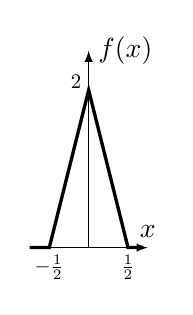
\begin{tikzpicture}
  \draw[-latex] (-0.75,0)--(0.75,0) node[above] {\(x\)};
  \draw[-latex] (0,0)--(0, 2.5) node[right] {\(f(x)\)};
  \draw[very thick] (-0.75,0) -- (-0.5,0)--(0,2)--(0.5,0)--(0.69,0);
  \node[below,scale=0.75] at (-0.5,0) {\(-\frac{1}{2}\)};
  \node[below,scale=0.75] at (0.5,0) {\(\frac{1}{2}\)};
  \node[left,scale=0.75] at (0,2.1) {\(2\)};
\end{tikzpicture}
\end{document}
